
\documentclass[10pt,a4paper]{article}

%%%%%%%%%%%%%%%%%%%%%%%%%%%%%%%%%%%%%%%%%%%%%%%%%%%%%%%%
%
% Packages and Theorem Environments

\usepackage{graphicx}
\usepackage{psfrag}
\usepackage{epsf}
\usepackage{amsmath,amsfonts,amssymb,latexsym}
\usepackage{enumitem}
\usepackage{algorithmic}
\usepackage{algorithm}
\usepackage[width=160mm,height=240mm,left=35mm,foot=10mm]{geometry}
\usepackage{xcolor}
\usepackage{url}
\usepackage{hyperref}
\usepackage{tikz}



\renewcommand{\theequation}{\thesection.\arabic{equation}}
\newcommand{\makeTiny}[1]{{\tiny #1}}
\newcommand{\work}{\tiny}
\newcommand{\ignore}[1]{}
\newcommand{\startClaims}{\setcounter{claim}{0}}
\newtheorem{theorem}{Theorem}[section]
\newtheorem{corollary}[theorem]{Corollary}
\newtheorem{lemma}[theorem]{Lemma}
\newtheorem{proposition}[theorem]{Proposition}
\newtheorem{conjecture}[theorem]{Conjecture}
\newtheorem{problem}[theorem]{Problem}
\newtheorem{question}[theorem]{Question}
\newtheorem{definition}[theorem]{Definition}
\newtheorem{task}[theorem]{Task}
\newtheorem{claim}{Claim}
\newtheorem{remark}[theorem]{Remark}
\newtheorem{observation}[theorem]{Observation}

\graphicspath{hw5}


\title{MATH 351--004 -- Assignment \#$5$\\
}

\author{Alex Iacob\\
ai9388}

\date{September 30, 2021}


%%%%%%%%%%%%%%%%%%%%%%%%%%%%%%%%%%%%%%%%%%%%%%%%%%%%%%%%
%
% Author's definitions


\newcommand{\NN}{\mathbb N}
\newcommand{\ZZ}{\mathbb Z}
\newcommand{\QQ}{\mathbb Q}
\newcommand{\RR}{\mathbb R}

\newcommand{\BB}{\mathcal B}
\newcommand{\ZT}{\mathcal Z}

\newcommand{\Cl}{\operatorname{Cl}}
\newcommand{\Bd}{\operatorname{Bd}}
\newcommand{\row}{\operatorname{row}}
\newcommand{\col}{\operatorname{col}}
\newcommand{\Span}{\operatorname{span}}
\newcommand{\convhull}{\operatorname{conv.hull}}
\newcommand{\tr}{\operatorname{tr}}

\newcommand{\diam}{\operatorname{diam}}

\begin{document}

\maketitle


\subsection*{Problem 1 -  Find a BFS tree and DFS tree for $K_{n, n}$}
(Sorry, not the best image, but writing this out in LaTeX seemed more difficult)\\
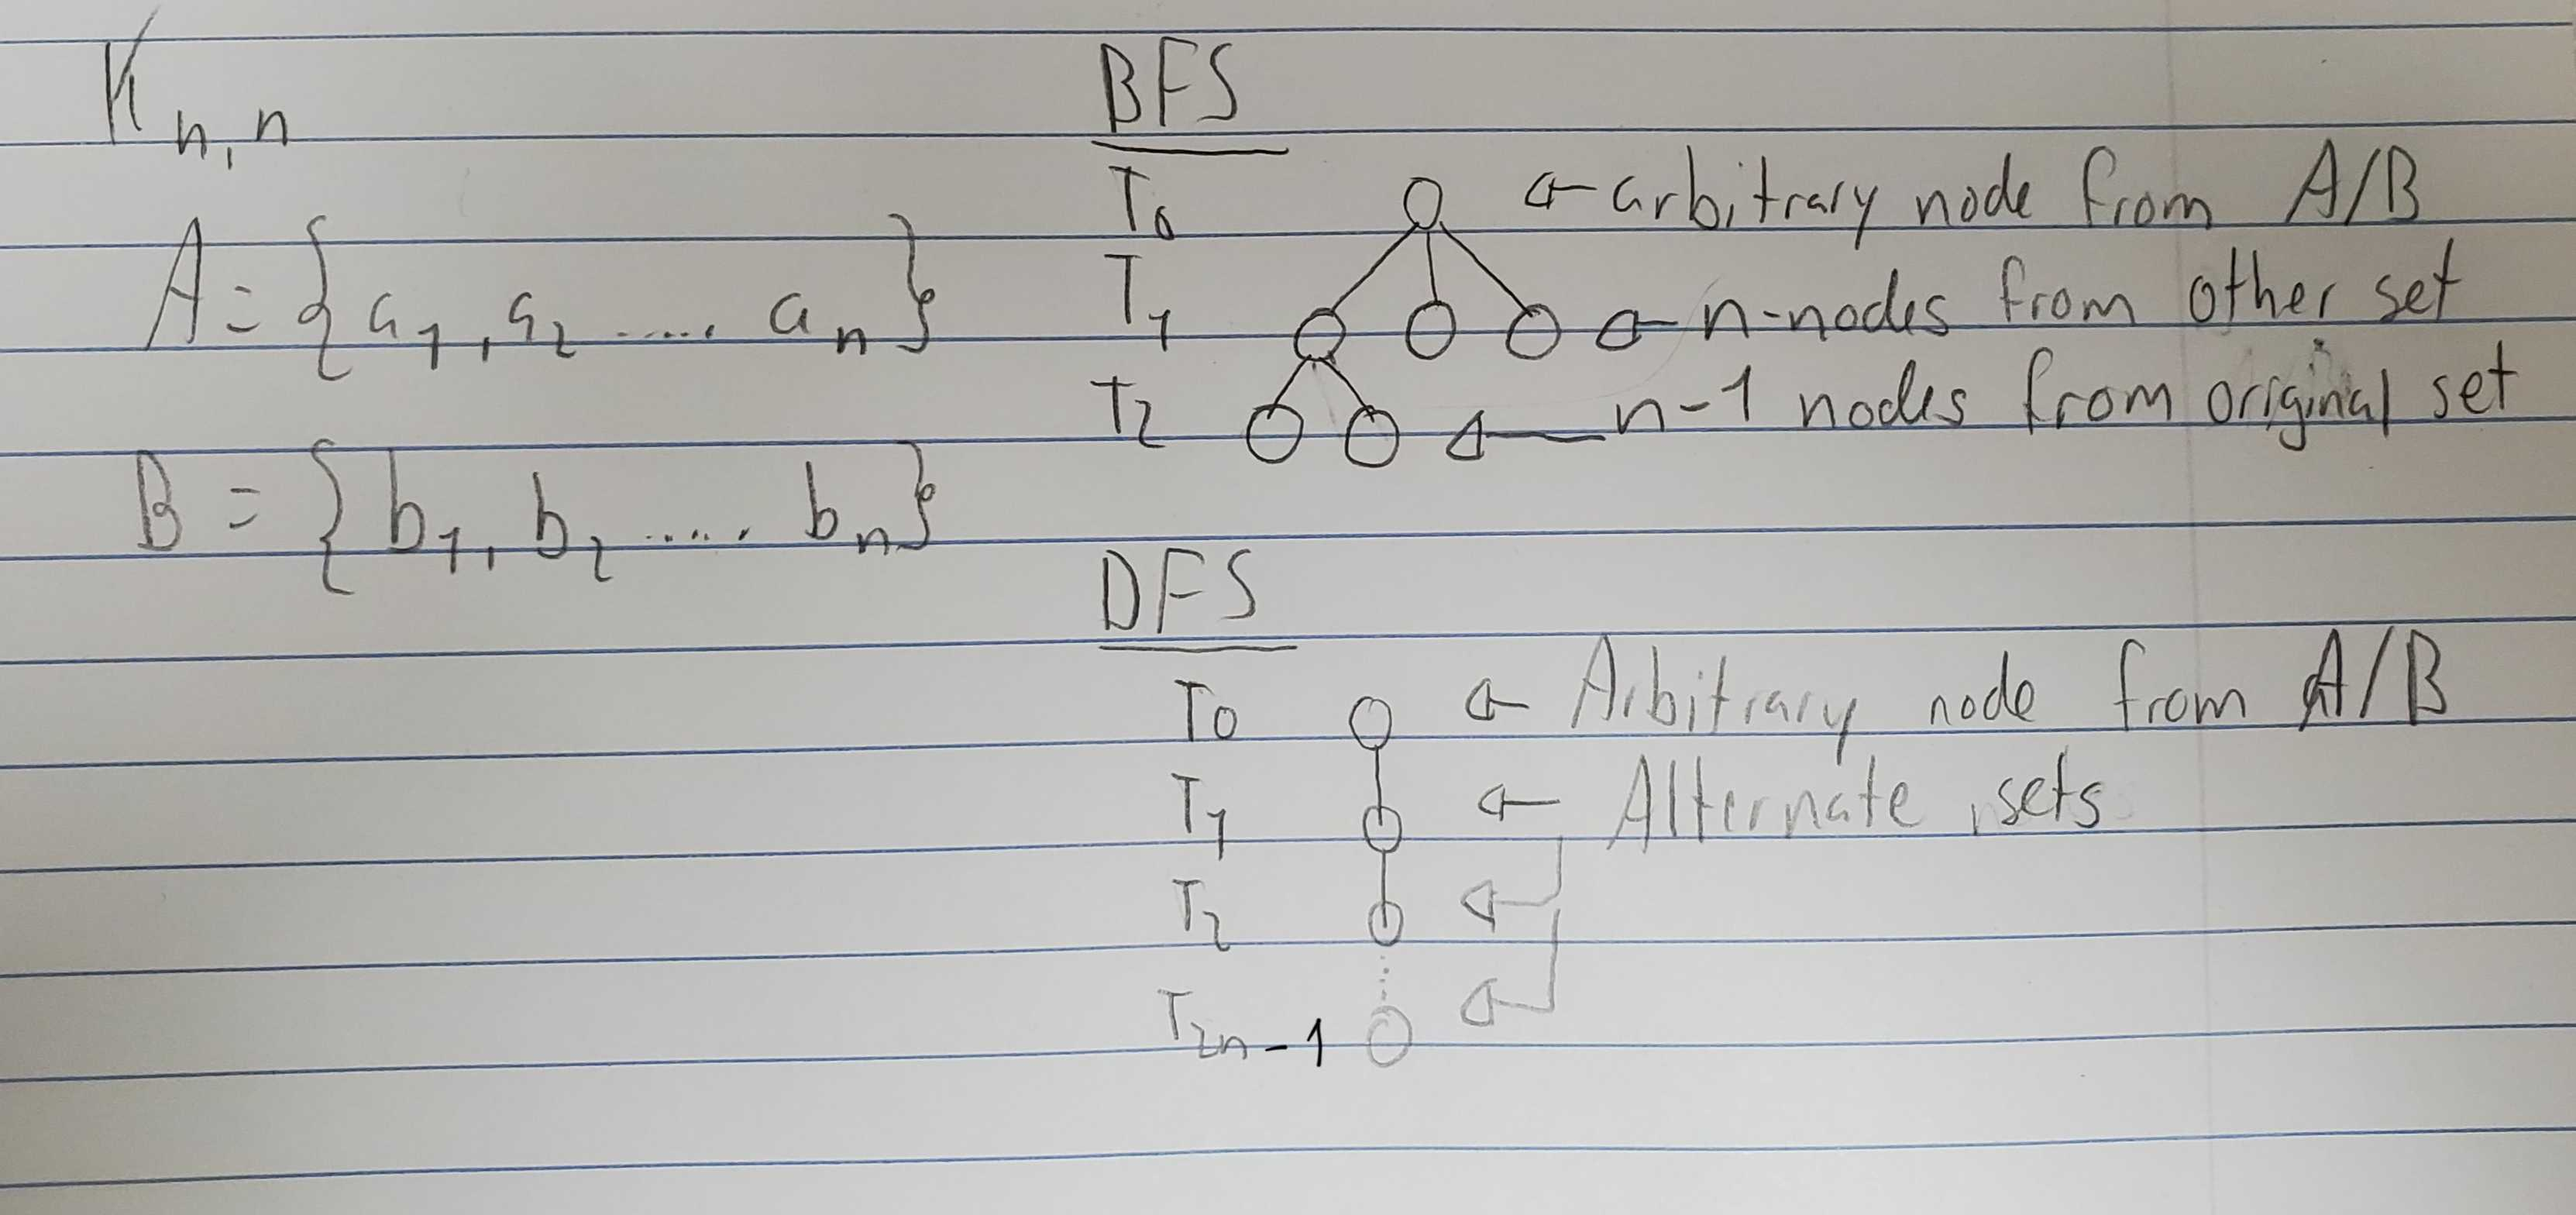
\includegraphics[width = 15 cm]{question1}

\subsection*{Problem 2 - Prove that an edge $e$ of a connected graph is a bridge if and only if $e$ belongs to every spanning tree of $G$}

Forward: A connected graph's edge is a bridge if it belongs to every spanning tree of the graph.\\
Contrapositive: Suppose that $e$ does not belong to every spanning tree of $G$. There exists spanning tree $T$ that does not contain edge $e$, therefore, tree $T$ is spanning subgraph $G - e$. Using Theorem 4.2, there are two arbitrary vertices, $u and v$ that have a unique uv-path in $T$ and $G - e$. This means that e is not a bridge.\\\\
Backward: An edge belongs to every spanning tree then it is a bridge in a connected graph.\\
Contrapositive: Suppose that $e$ is not a bridge, then we know that $G - e$ is connected and has spanning tree $T$. Since $G - e$ has the same vertices as $G$, then $T$ does not contain edge $e$.

\subsection*{\newpage Problem 3 - Apply both Kruskal's and Prim's algorithms to find a minimum spanning tree in the weighted graph in figure 4.12. In each case, show how this tree is constructed, as in Figures 4.5 and 4.9}
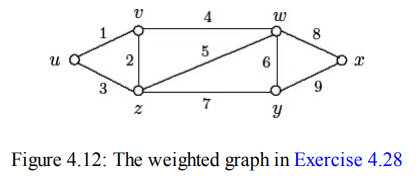
\includegraphics[width = 7cm]{fig412}\\
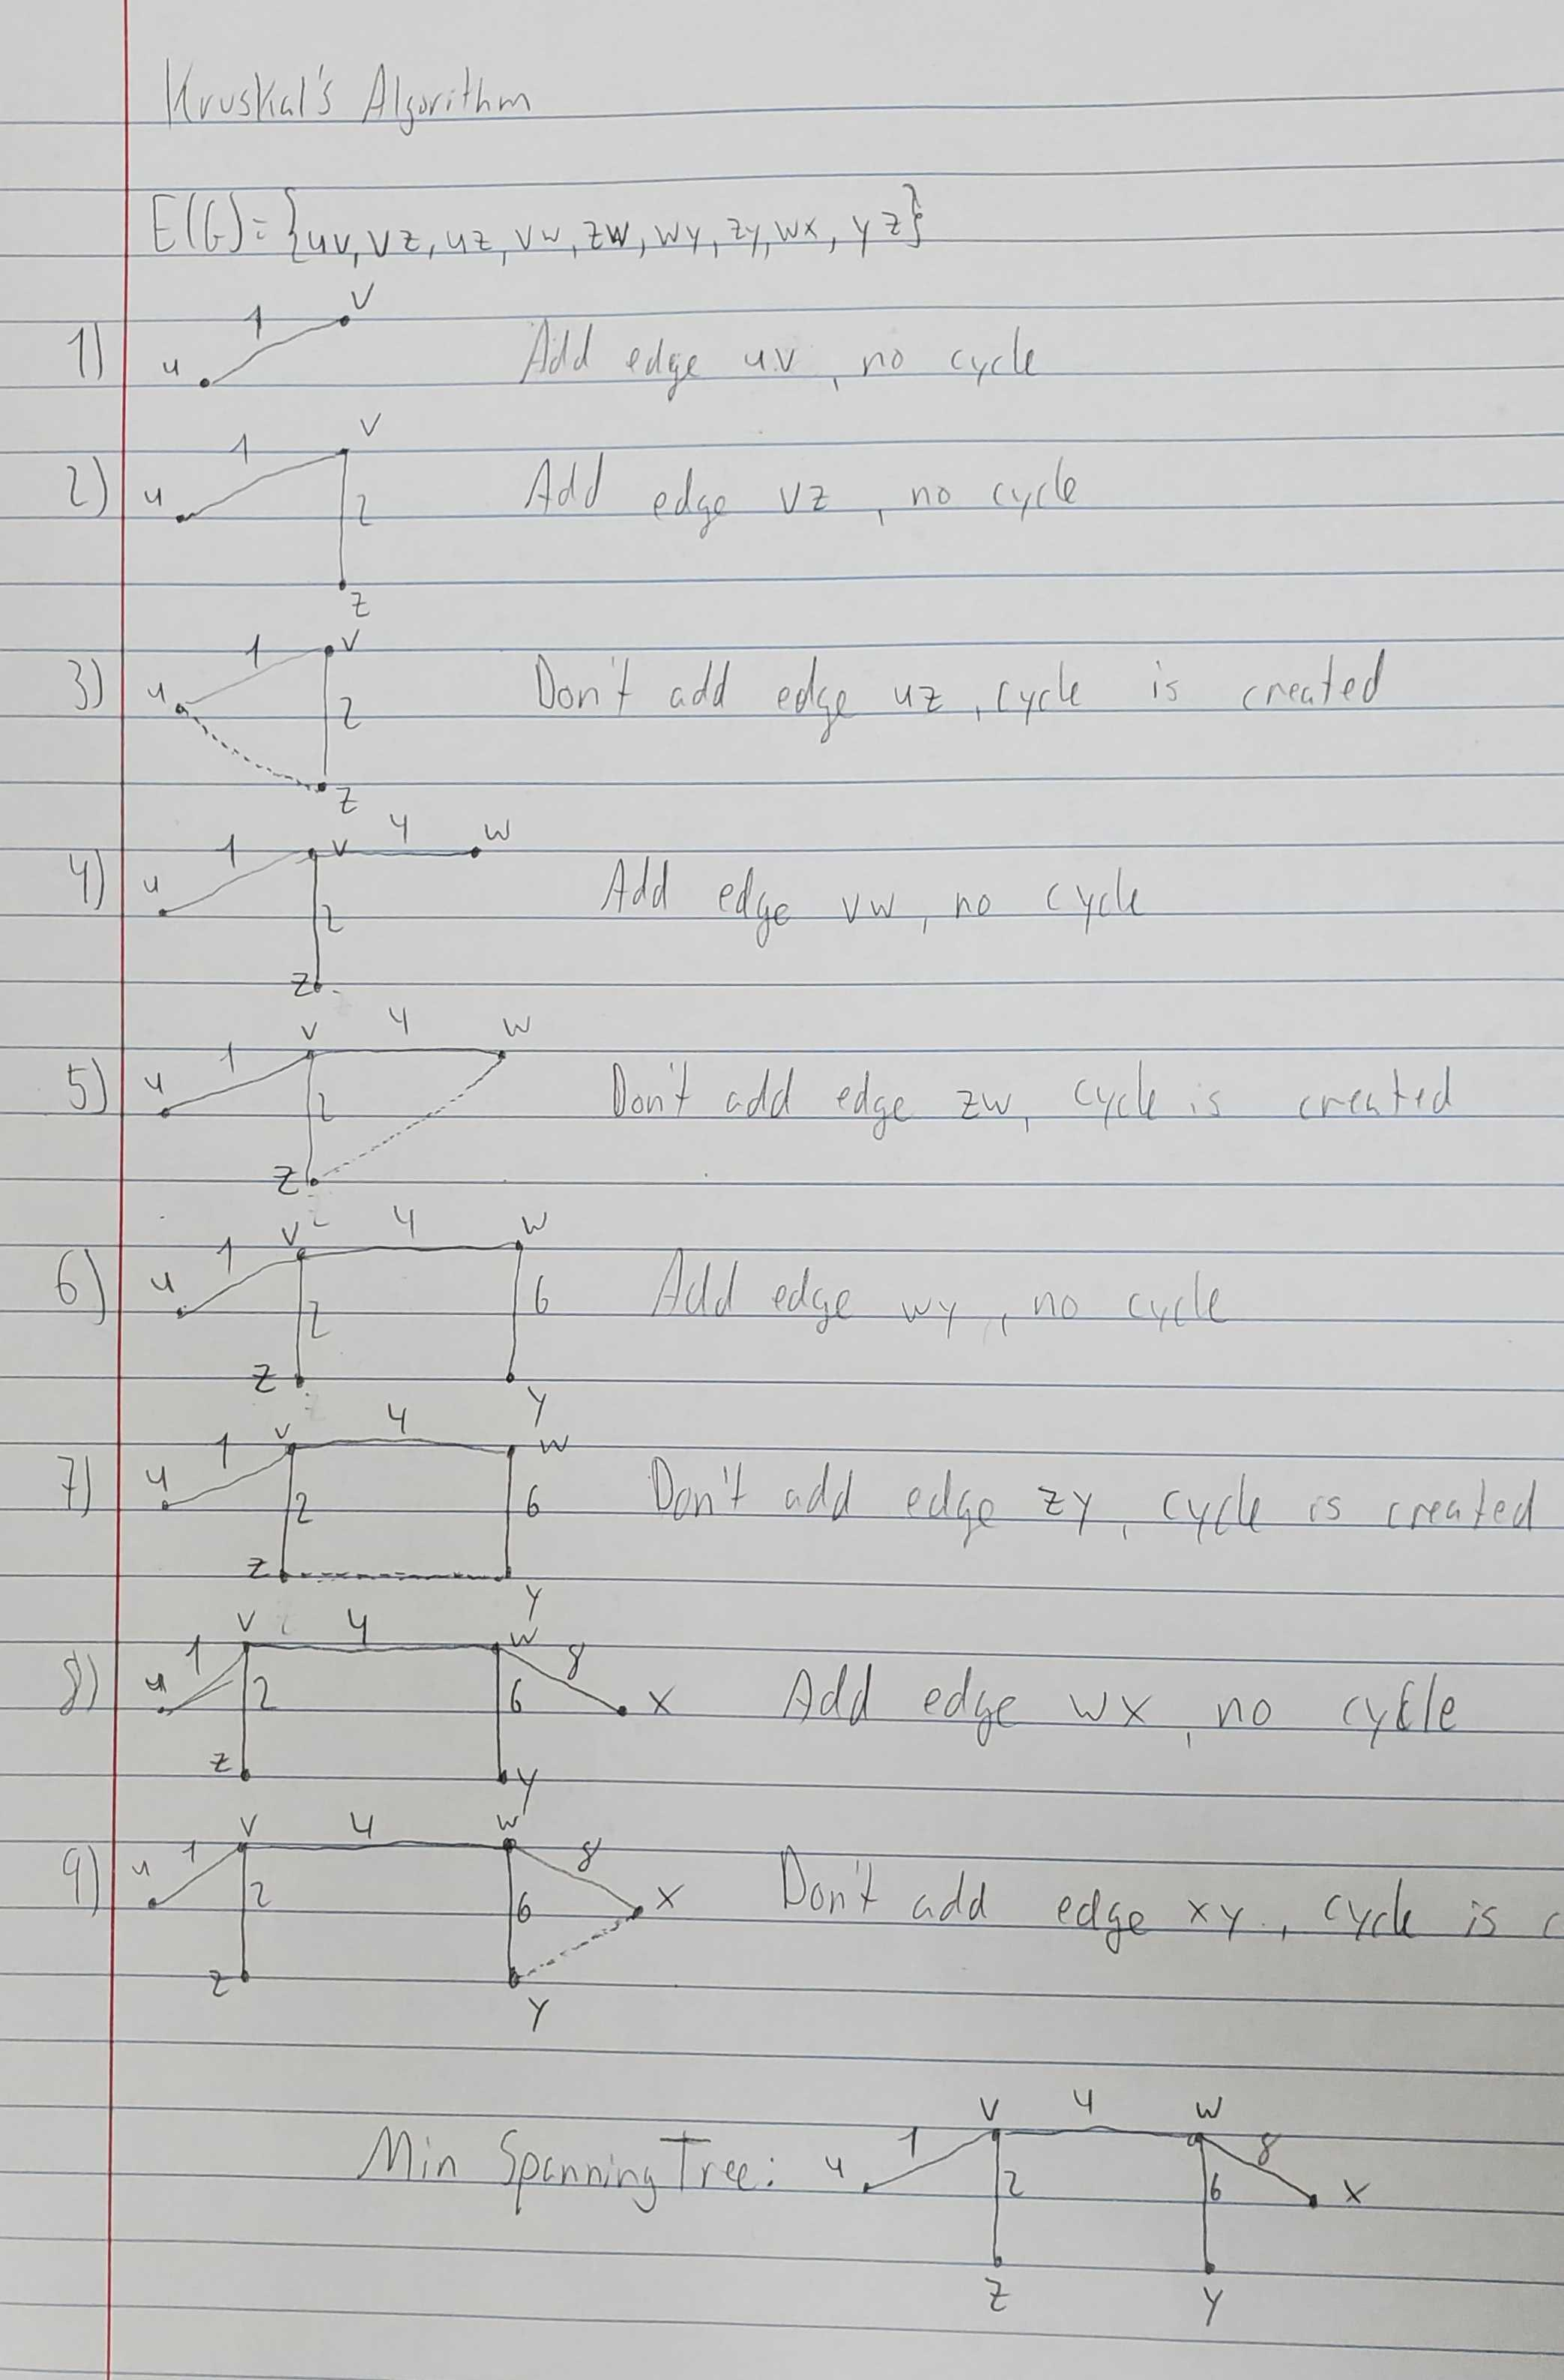
\includegraphics[width = 11cm]{kruskals}\\
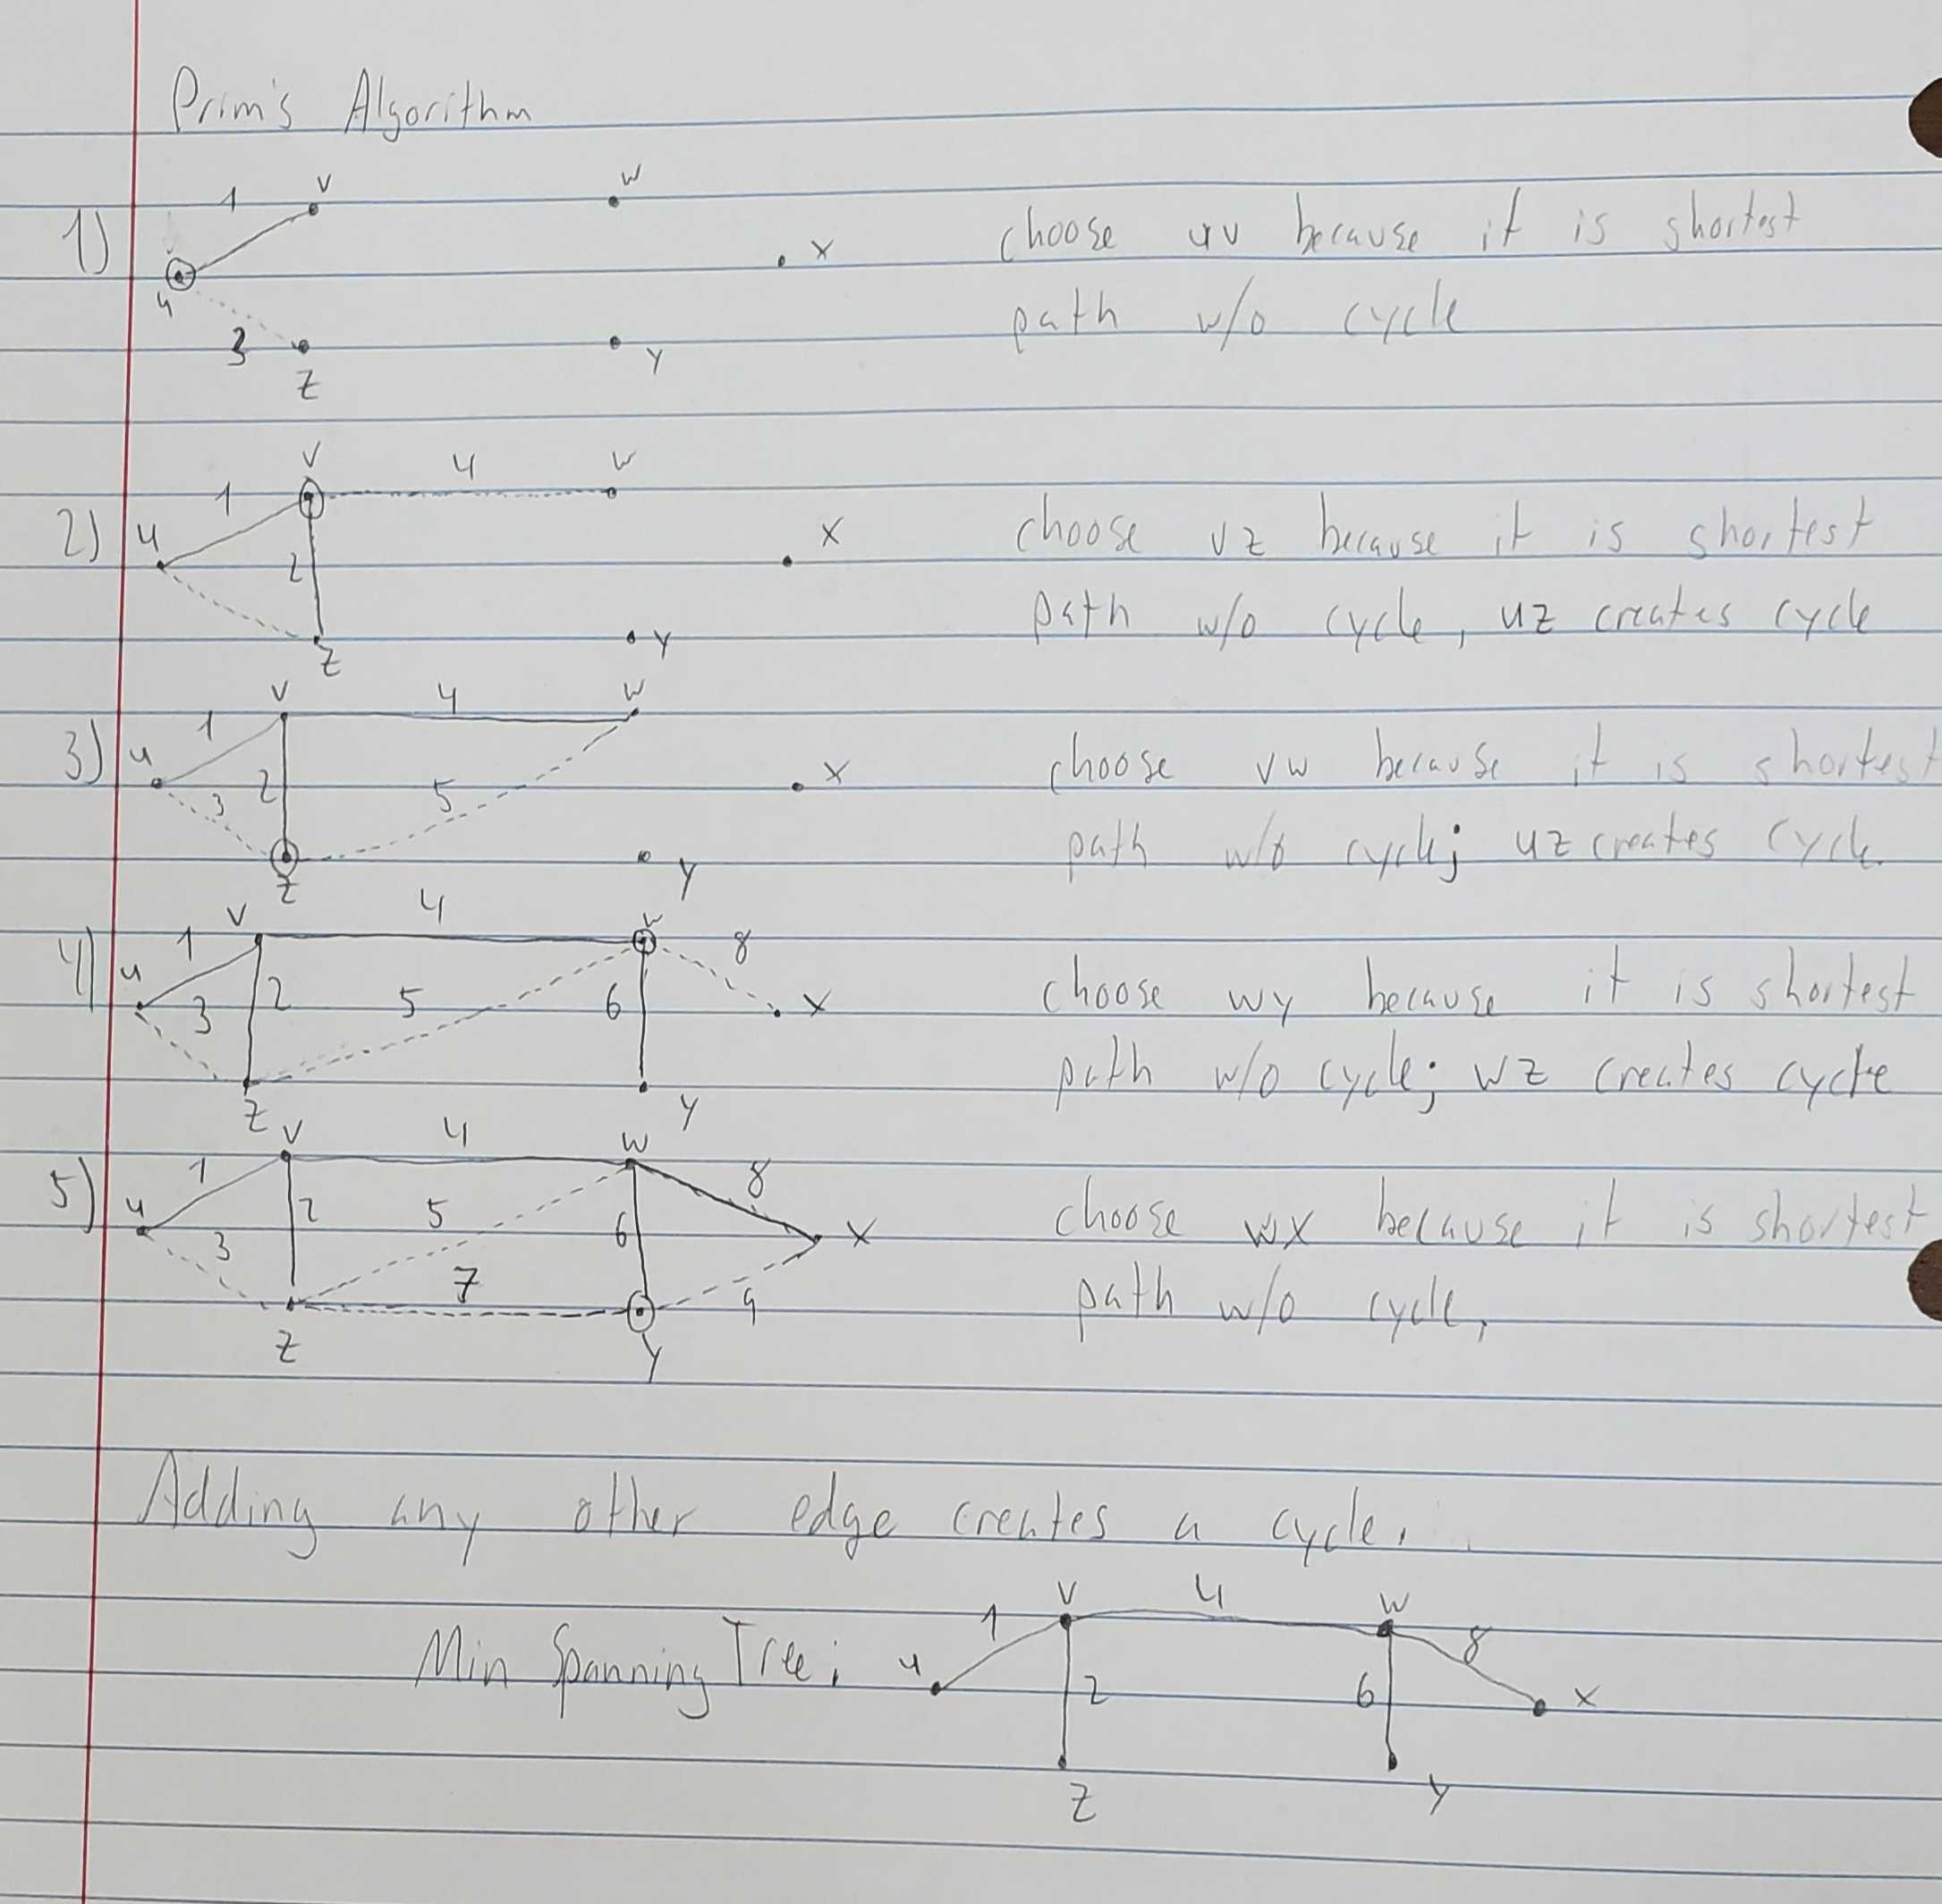
\includegraphics[width = 11cm]{prims}\\

\subsection*{Problem 4 - Let $G$ be a connected weighted graph and $T$ a minimum spanning tree of $G$. Show that $T$ is a unique minimum spanning tree of $G$ if and only if the weight of each edge $e$ of $G$ that is not in $T$ exceeds the weight of every other edge on the cycle in $T + e$}
Suppose that $T$ is a unique minimum spanning tree of $G$. Let $e$ be an edge which is not in $T$, which means that $T + e$ contains a cycle $C$. \\ Suppose that there exists another edge $d$, such that its weight is greater than $e$, $w(e) < w(d)$. We can create another spanning tree $T\prime = (T - e) - d$. Since we know what $w(e) < w(d)$, this means that $W(T) > W(T\prime)$ Contradiction\\




\end{document} 




















